
\documentclass[12pt]{article}
\usepackage{geometry} % see geometry.pdf on how to lay out the page. There's lots.
\geometry{a4paper} % or letter or a5paper or ... etc
\usepackage{bm} % see geometry.pdf on how to lay out the page. There's lots.
\usepackage{amsmath}
\usepackage{graphicx}
\usepackage{pdflscape}
\usepackage{subcaption}
\usepackage[round]{natbib}
\usepackage[font=small]{caption}
\usepackage[labelformat=empty, position=top]{subcaption}
\usepackage{authblk}
\usepackage{setspace}
\usepackage{hyperref}
\usepackage{color}
\newcommand{\sinead}[1]{{\color{green} #1}}
% \geometry{landscape} % rotated page geometry

% See the ``Article customise'' template for come common customisations

%%% BEGIN DOCUMENT
\begin{document}

\title{Selective constraints on global plankton dispersal}

\author[1,*]{B.A. Ward}
\author[2]{B.B. Cael}
\author[3]{S. Collins}  
\author[2]{C.R. Young}

\affil[1]{\small{Ocean and Earth Science, University of Southampton, Southampton, UK} }
\affil[2]{\small{National Oceanography Centre, European Way, Southampton, UK} }
\affil[3]{\small{Institute of Evolutionary Biology, School of Biological Sciences, University of Edinburgh, Edinburgh, UK} }
\affil[*]{\small{Corresponding author: b.a.ward@soton.ac.uk}}

\date{} % delete this line to display the current date

 

\maketitle
\onehalfspacing

\section*{Abstract}


\section*{Introduction}

Marine microbial communities are highly interconnected assemblages of organisms shaped by ecological drift, natural selection and dispersal. The relative strength of these forces determines how ecosystems respond to environmental gradients, how much diversity is resident in a community or population at any given time, and how populations reorganise and evolve in response to environmental perturbations \citep{?}. Over evolutionary timescales, the outcome of these processes will affect community assembly through diversification, ecosystem function through biogeochemical cycling, and ultimately the resilience of marine ecosystems to environmental change \citep{?}. Therefore, understanding the mechanisms that lead to niche diversification and biogeographic structure in microbial communities is a fundamental pursuit of marine microbial research \citep{?}. A central question is to what degree are biogeographic patterns attributable to local selection based on contemporary environmental factors, or to independent stochastic processes occurring in geographic-isolated regions \citep[Figure~\ref{HughesMartiny} and][]{Hughes-Martiny:2006}. 

Recent analysis of metagenomic data \citep[Figure~\ref{Richter_Tara} and][]{Richter:2019}, has shown that large-scale trends in community composition are correlated both with environmental variables and community composition, with distinct clusters emerging along environmental gradients and among the most closely connected sites. When sample sites are clustered based on Jaccard dissimilarity of operational taxonomic units, there is discernible ecological similarity among sites within the the same ocean basins (Figure~\ref{Richter_Tara}a), although we also see sites within the same ocean basin clustered far apart and sites from geographically remote locations clustered together (Figure~\ref{Richter_Tara}b). The broad patterns appear to reflect geographic proximity, and perhaps to a lesser extent, environmental selection \citep[][and Figures~\ref{Tara_HughesMartiny} and~\ref{Tara_Dendrogram}]{Richter:2019}. Nonetheless, the mechanisms underlying the observed biogeography remain uncertain. The roles of selection and dispersal have both been examined using global-scale models, but typically with one in isolation from the other. On one hand, population dynamic models have focused on the role of selection from among a universal background of candidate species \citep{Follows:2007}. This is the view framed in the \citet{BaasBecking:1934} hypothesis: `everything is everywhere, but the environment selects'. On the other hand, a number of studies have addressed the question of global gene flow in oceanic microbial communities, using particle tracking models to assess connectivity through the surface waters \citep{Hellweger:2014,Jonsson:2016}, but these have typically assumed ecological neutrality \citep{Hubbell:2001}, and have thus ignored the role of selection. While some studies find that the ocean surface is very rapidly connected on timescales of decades or less \citep{Jonsson:2016}, others suggest that current rates of passive dispersal are insufficient to overcome biogeographic differences created by chance mutations occurring in geographically isolated regions of the ocean \citep{Hellweger:2014}.

\sinead{I would argue that the "everything is everywhere and the environment selects" needs to be broken down into first, can everything get everywhere, which is a (relatively) simple matter of connectivity that treats cells as passive particles. The second bit is given that a genotype arrives at a given location, can it grow? This requires including selection, which breaks down into first, is that patch already occupied by someone with higher fitness, and second, if not, is the fitness advantage,population size, and invasion frequency of the invader high enough to invade from rare - is the invading population likely to escape stochastic loss while relatively rare? (I think we need to spell out all the moving parts in the "everything is everywhere and the environment selects"  idea, because it is not as simple as it sounds).}

\begin{figure*}[t!]
    \centering
        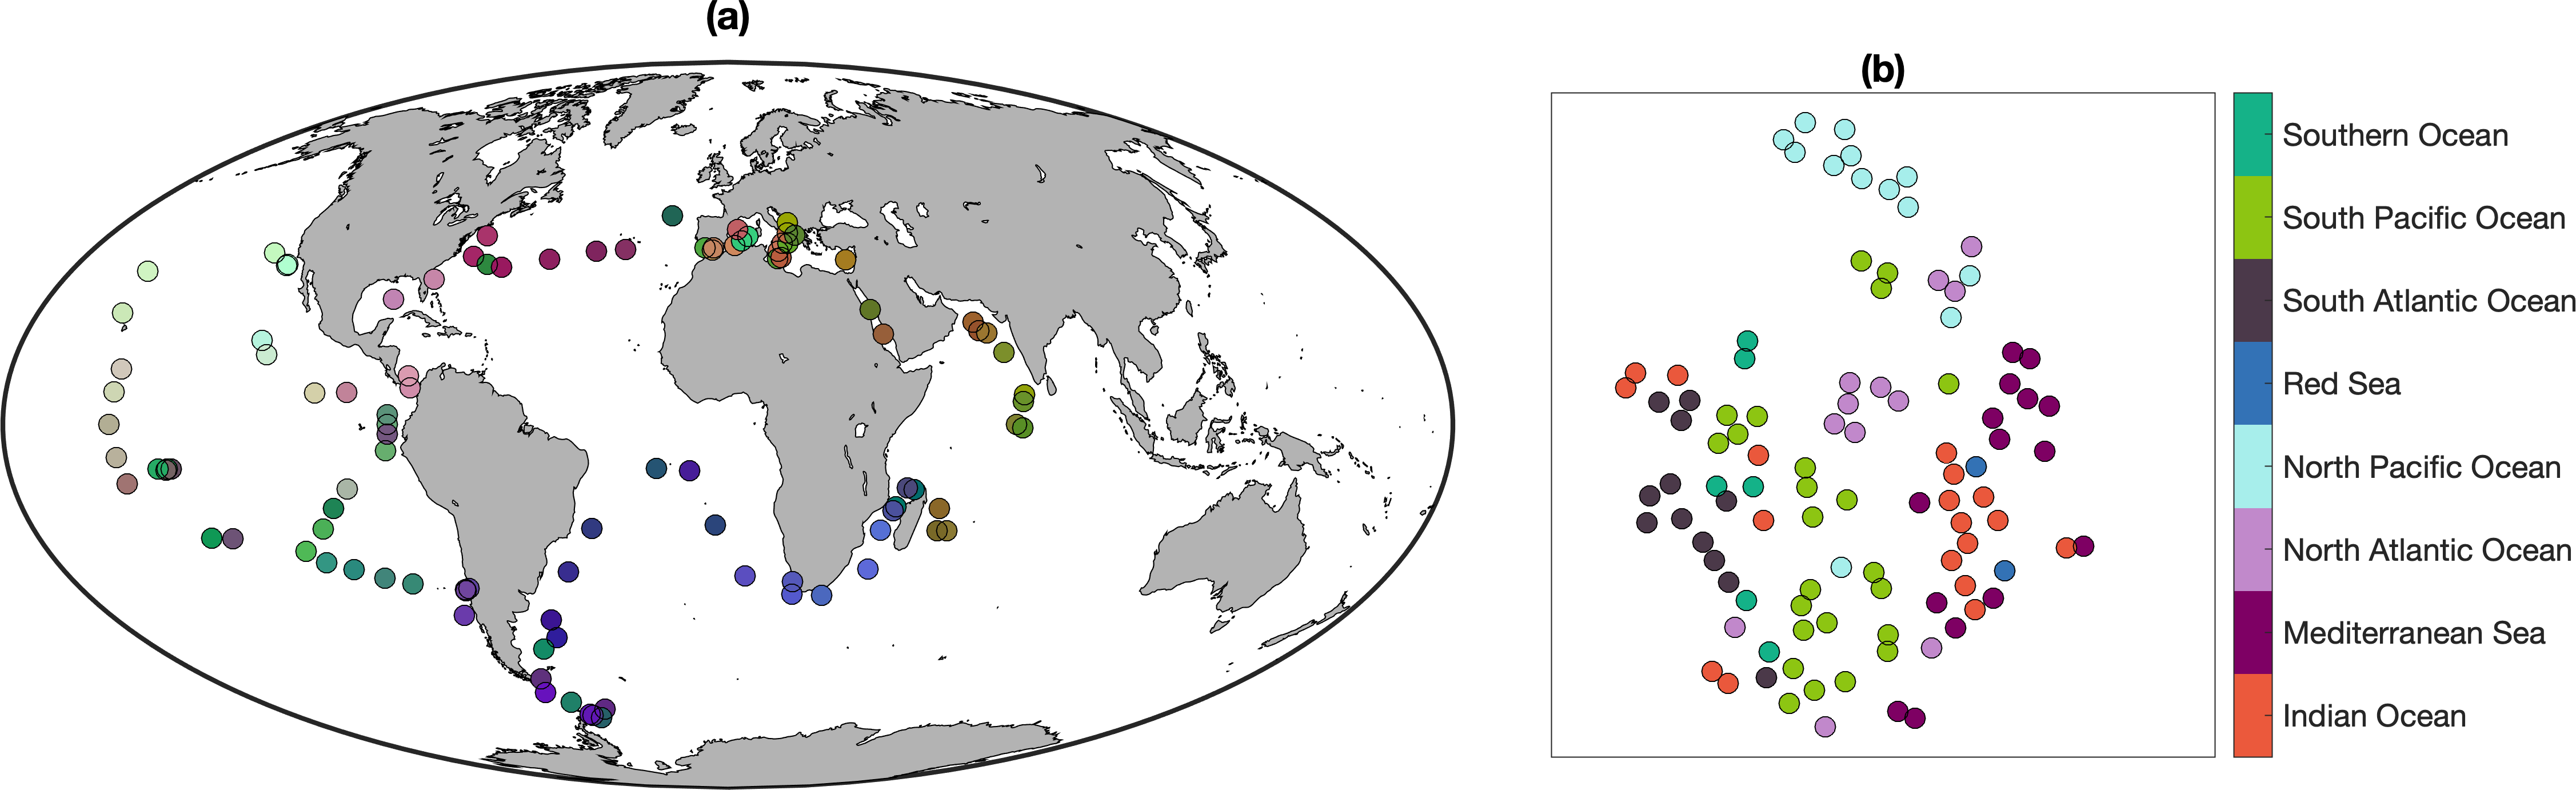
\includegraphics[width=1\textwidth]{../Richter_2020_Tara_data/Figures/Richter_OTU_cluster_3.png}\
    \caption{Taxonomic community similarity clusters in the 0.8 - 5 $\mu$m size fraction across \textit{Tara Oceans} sites \citep[replotted using data from][]{Richter:2019}. (\textbf{a} and \textbf{b}) Community similarity is shown with colours by projecting the Taxonomic Jaccard dissimilarity matrix into the `rgb' colour space using the t-SNE dimension-reduction algorithm \citep{VanDerMaaten:2014}. (\textbf{b}) Site $x$ and $y$ coordinates (dimensionless) are based on a 2-dimensional projection using the same algorithm.}
\label{Richter_Tara}
\end{figure*}

In order to distinguish between the biogeographic effects of selection and dispersal, we need a framework that accounts for both processes together. In a case where global dispersal is fast relative to competitive exclusion, we should expect community composition to always reflect the local environmental conditions \sinead{and for local composition to be largely predictable from environmental conditions in the absence of strong barriers to invasion imposed by local adaptation.}  (Figure~\ref{HughesMartiny}). \sinead{However, the relative rates of dispersal and competitive exclusion will depend on physical dispersal rates in the first instance and differences fitness between local populations and invaders in the second, with larger fitness differences (stronger local adaptation) decreasing both the probability and rate of invader success for a given amount of physical dispersal.}In the alternative case with limited connectivity between ocean regions, we should expect a more unpredictable community structure in any given location \sinead{regardless of the ability of populations to adapt to their local conditions}, with geographically-isolated but otherwise similar environments displaying significant differences in their taxonomic composition.

In this paper, we develop a population genetic model representing a single clonally-reproducing plankton population, embedded within an empirically-constrained representation of ocean circulation. In contrast to previous studies, our model accounts for population size, stochastic demography, natural selection, adaptation and transport through the ocean interior. We find that estimates based on dispersal pathways restricted to the ocean surface markedly underestimate global connectivity. With a more realistic transport term accounting for dispersal at all depths, we find that varying the degree of selection and adaptation leads to very different model outcomes in terms of community biogeography and global connectivity. We show that \sinead{accounting for the ability of populations to adapt to  their thermal environment allows} selection based on thermal niches \sinead{ to act} as a major constraint on dispersal \sinead{by favoring locally adapted populations even in the face of invaders being introduced by mixing}, with the clear effects on biogeographic organisation at the global scale.  

%One criticism of these approaches is the large difference between the modelled global population size (10$^5$ agents) and the estimated global census population size $N_c \approx 10^{27}$. Some authors have argued that Prochlorococcus subpopulation effective size, $N_e$, is close to the census size \citep{Kashtan:2014}, but others disagree estimating an $N_e$ with an upper bound of 10$^7$ for \textit{Prochlorococcus} \citep{Price:2015} or a range on the order of 10$^8$-10$^9$ for a broad range of taxa \citep[n=153,][]{Bobay:2018}. Many factors can cause $N_e << N_c$ such as population fluctuations \citep{}, a large variance in reproductive success \citep{Eldon:2006}, and background selection \citep{Good:2014,Kaiser_2009}. Determining the effect of $N_e$ and the sensitivity of model predictions to a range of $N_e$ would be useful.

% In order to understand the effects of natural selection, we will have to make some assumptions about the mutation process, the distribution of selection coefficients that this process generates, and the mapping of these genetic mutations to phenotypes such as temperature tolerance. There are many examples of gene variants in marine taxa that respond to thermal gradients due to amino acid replacements (reviewed in Somero 2010). This class of mutations affects the thermodynamic stability of proteins and is likely responsible for evolutionary innovations as well as pleiotropic or genotype x environment effects (Depristo 2007). However, mutations can also contribute to evolutionary innovation (or cell death) through gene loss or effects on gene regulation (inversions, frame shifts, mobile elements, etc.). For example, populations of the coccolithophore Emiliania huxleyi have recently been shown to have lost 1N-specific genes resulting in rather rapid and profound alterations of life history (Dassow et al. 2015). Hypermutability is a phenotypic state that many single-celled organisms transition to under conditions of stress (). The distribution and rate of the various classes of mutations occurring in phytoplankton is currently not well constrained (????). The error threshold theory suggests that one mutation per genome per generation should be the upper limit of mutational input (Drake….), but this theory is violated (at least by) some viruses (Lauring et al. 2010). 

%One of the challenges of estimating $N_e$ in microbial populations is the difficulty of defining bacterial species. A study utilizing single-cell genomics revealed hundreds of coexisting subpopulations of Prochlorococcus that cluster based on shared genotypes in the majority of core genes associated with a small set of distinct flexible genes linked to that backbone \citep{Kashtan:2014}. The community composition of these subpopulations fluctuate seasonally, suggesting that they are ecologically distinct. These clusters likely correspond to ecotypes as defined by \citep{Cohen:2001} ecologically equivalent subpopulations through which selective sweeps of an adaptive mutant outcompetes all other strains of that subpopulation. \citet{Kashtan:2014} argue that the census size of these subpopulations in well-mixed water parcels (10km$^2 \times$ 3m) is likely greater than 10$^13$ cells and close to the census size. Interestingly, on seasonal time scales, the total abundance of Prochlorococcus does not change, but the relative frequency of the subpopulations does, suggesting that the carrying capacity of the local environment applies to the collection of subpopulations \citep{Kashtan:2014}.

%Diatoms, on the other hand, are unicellular eukaryotes that can generally be characterized as having a diplontic life cycle, meaning that diploid (2 chromosome copies per cell) phases of the life cycle grow, but the haploid (single copy) do not (Chepurnov et al. 2004). The diploid phase reproduces by asexual mitotic division, whereas the haploid phase doesn’t reproduce, but allows recombination and shuffling of chromosome copies among lineages, i.e., sex. The rates and variability of asexual versus sexual reproduction in natural populations are currently not well-constrained. These life history characteristics are likely to have profound consequences for the creation and maintenance of genetic variation in natural populations and, hence, the ability of these taxa to weather global change. Cells may also enter a quiescent stage, forming resting spores that could facilitate dispersal in adverse conditions (Von Dassow et al. 2011). 

\section*{Simulations}

To assess the rate of planktonic dispersal across the global ocean, we developed a model that tracks the relative abundances of adapting subpopulations in a globally distributed metapopulation, with spatially varying carrying capacity, $\mathbf{N}$. At the beginning of each simulation, a resident subpopulation is assumed to have population frequency of 1 throughout the global ocean. However, at each of 94 `seed locations' distributed more or less evenly around the ocean (dots in Figure~\ref{Connectivity_map_pro}), the resident subpopulation is replaced with a taxonomically distinct (but ecologically identical) local subpopulation. From this initial condition, the model is integrated for 100 years in discrete time. Every six hours, plankton cells are dispersed by the ocean circulation. Every 24 hours the population is replaced with a new generation of $\mathbf{N}$ cells, drawn at random from the existing generation, with probabilities given by the relative abundance of each subpopulation and, where appropriate, a temperature-dependent selection coefficient, $s$ \citep{Cherry:2003}. In regions where a subpopulation is present in high abundance, this stochastic process has no significant effect on the relative abundance, but it introduces a meaningful chance of local extinction wherever abundances are low (such as at edges of a subpopulation's range). 

Our main set of simulations tracks the dispersal of a globally-abundant \textit{Prochlorococcus} population with a cellular diameter of approximately 0.6 microns, setting $\mathbf{N}$ to the depth-integrated cellular abundance within each grid box \citep{Dutkiewicz:2019}. The results presented below are derived from from simulations based on a single repeating year with time-invariant environmental temperatures and population carrying capacities. We also performed simulations where these variables followed a seasonal cycle, finding that the results were not overly sensitive to the change (Figure~\ref{Cumulative}).

\paragraph{Ecologically neutral dispersal by surface transport.}

We initially considered a scenario where cells are transported exclusively within the surface layer, with all subpopulations equally well adapted at all temperatures \citep[i.e. ecologically neutral;][]{Hubbell:2001}. The dark blue lines in Figure~\ref{Cumulative}a show the timescales over which the 94 \textit{Prochlorococcus} seed subpopulations reach the rest of the ocean. Largely in agreement with \citet{Jonsson:2016}, almost 90\% of the surface ocean is connected within a decade. %However, Figure~\ref{Cumulative}b indicates that the diatom population is much less well-connected, with less than 50\% connectance after 100 years. The difference in global connectance between the \textit{Prochlorococcus} and diatom populations is attributable to the different carrying capacities. Whereas the \textit{Prochlorococcus} population is globally ubiquitous and extremely abundant (Figure~\ref{Abundances}a), the diatom population is much less abundant, with large regions of the surface ocean where it is effectively absent (Figure~\ref{Abundances}b) providing significant barriers to dispersal. This highlights that the likelihood of dispersal pathways is a critical factor that should not be overlooked when estimating global dispersal. 

\begin{figure*}[htp!]
    \centering
        \includegraphics[width=0.75\textwidth]{../Figures/Figure_1.png}
\caption{Fraction of connections between the 94 seed locations and the rest of the ocean through time. Solid lines show the results of simulations with time-invariant temperatures and carrying capacities. Dashed lines show the results of simulations with seasonally varying temperature and carrying capacity.}
\label{Cumulative}
\end{figure*}

The global dispersal of the ecologically neutral subpopulations is broken down further in Figure~\ref{Connectivity_map_pro}a. Here immigration times (background colours) suggest that temperate latitudes are generally more easily invaded than the equatorial regions. Conversely, emigration times (coloured dots) suggest that subpopulations initialised at lower latitudes are more rapidly dispersed throughout the ocean than those from higher latitudes. Plotting immigration times against emigration times for the `surface-only' simulation (Figure~\ref{Imm_vs_em}) confirms that low latitudes act as source regions, with slow immigration and fast emigration, while high latitudes act as sink regions, with fast immigration and slow emigration.

These regional differences in immigration and emigration timescales are explained by the surface circulation patterns shown in Figure~\ref{Connectivity_map_pro}a. The two-dimensional surface transport vectors are highly divergent in equatorial upwelling regions, driving a consistent efflux of cells that must be topped up to the carrying capacity by reproduction of the local resident population. These regions thus export cells to the rest of the ocean, while remaining resistant to immigration. The sub-tropical gyres, meanwhile, are characterised by convergent flow, with a consistent influx of cells diluting the local resident populations. These regions are thus easily invaded and are slower to export cells to the rest of the ocean. 

%However, the less abundant and more sparsely distributed diatom population is much less well connected, with less than 50\% of sites connected after 100 years. Figure~\ref{Abundances}b shows that this is attributable to greatly diminished or non-existent fluxes through the oligotrophic gyres, where diatom abundance is extremely low. 


\begin{figure*}[htp]
\centering
\includegraphics[width=0.6\textwidth]{../Figures/Figure_2.png}
    \\
    \caption{Immigration and emigration timescales (years) for ecologically neutral \textit{Prochlorococcus} subpopulations, given (a) surface only transport, and (b) depth-integrated transport. Taxonomically distinct subpopulations were seeded in each of the 94 locations marked with dots. Emigration times, represented by the coloured dots, are defined as the time taken for each seed subpopulation to disperse to 95\% of all locations). Immigration times, represented by the background colours, are defined as the time taken for 95\% of all seed subpopulations to arrive in each location. Planktonic transport velocities are shown as vectors. (c) Relative changes in global immigration and emigration times when switching from surface-only to depth-integrated transport (b$\div$a).}
\label{Connectivity_map_pro}
\end{figure*}

\paragraph{Depth-integrated transport.}

The assumption that horizontal dispersal of plankton occurs only in the surface layer ignores the potential role of subsurface connectivity. To test the sensitivity of our results to this pathway, we calculated the depth-integrated horizontal transport of cells across the entire water column, weighting transport fluxes at each depth by the local population abundance. After this adjustment to the transport component, we repeated our initial experiment in the same way. 
Allowing for sub-surface transport slightly accelerates global plankton dispersal (pale blue line in Figure~\ref{Cumulative}), with more than 97\% of the ocean connected in less than a decade. Spatially, the global distribution of immigration and emigration times has decreased everywhere (Figure~\ref{Connectivity_map_pro}), with the the differences in timescales between source and sink regions largely obliterated in the less divergent depth-integrated flow field (black dots in Figure~\ref{Imm_vs_em}). 

\paragraph{Selection between types.}

The previous experiments have assumed that all subpopulations are equally well-adapted to conditions throughout the entire ocean, but we know that changing conditions select for different phenotypes along environmental gradients \citep{Tilman:1990,Thomas:2012}, and that dispersing populations will be selected against as they stray beyond their optimal environments. \sinead{One component of natural selection is genotype sorting, where more fit types can replace less-fit ones.}

To test the influence of these effects \sinead{replace "these effects" with "genotype sorting based on standing variation"}, we focussed on a single trait, assigning thermal tolerance curves such that populations are preferentially selected when ambient temperatures align with their thermal optima (Equation~\ref{selection_TPC}). Each seed population is assigned a thermal optimum matching the average temperature at its initial location. At the same time, the global resident population is divided into 77 subpopulations, each with thermal optima matching the average temperature at its initial location \sinead{which is consistent with the existence of locally adapted resident populations, but ignores the ability of genotypes to themselves evolve over time (see next section) - might be worth noting that genotypes sorting without mutation is how most ESMs represent evolution???}. The model was then evaluated with the depth-integrated circulation scheme.

The global dispersal of the 94 seed populations is severely restricted by temperature-based selection (green line in Figure~\ref{Cumulative}), with global connectivity not rising above 15\% in the 100 year simulation. 

\paragraph{Adaptation within types.}

Temperature-related selection places a strong constraint on the dispersal of thermally-adapted populations. If populations are to overcome this restriction, they must adapt \sinead{dynamically} to their  environments \sinead{by generating heritable phenotypic changes over time} \citep{Thomas:2012,ODonnell:2018}. We included this capacity in the model by allowing all subpopulations to produce a small fraction of mutants \sinead{I would replace "mutants" with "offspring" and add the following, possibly in SI: this incorporates a large range of molecular mechanisms, including plastic and heritable plastic responses, standard mutations, sex, and horizontal gene transfer.} with different thermal optima (see SI-Methods). We initialised the experiment as before, with each subpopulation optimally adapted to its local temperature, but allowed for a small mutational flux \sinead{maybe call it trait diffusion rate or flux?} between adjacent phenotypes \citep{Sauterey:2017,Beckmann:2019}. \sinead{In line with previous validated studies,}We performed simulations with mutation rates of 1\% and 10\%. \sinead{I think that Beckmann does a good job of justifying why trait diffusion mutation rates look so high relative to point mutation rates or per-site substitution rates, so we should just cite them and move on... but we could call it a "trait diffusion rate" rather than a "mutation rate", which I think is a more apt description of what we're actually representing. Still, 10\% is high, and we could couch it as a proof of principle showing that you still get local adaptation hindering population homogenization, and that the actual effect is likely to be more severe, in line with the 1\% trait diffusion rate}

Even with an extremely high mutation rate of 10\%, global dispersal is markedly restricted by selection effects, with 95\% connectivity only achieved after approximately 30 years (orange line in Figure~\ref{Cumulative}). When the mutation rate is set to 1\%, just over 30\% of the ocean has been connected within 100 years (yellow line in Figure~\ref{Cumulative}). 

The global distributions of an illustrative seed population, 100 years after it was initialised in the central North Atlantic (35$^\circ$N, 46$^\circ$W) is shown in four illustrative cases in Figure~\ref{disperal_NA}. In the neutral model the highlighted population has complete global coverage, with highest concentrations in the Atlantic subtropical gyres (Figure~\ref{disperal_NA}a). Without selection, all seed populations are globally dispersed after 100 years, and community similarity appears to change smoothly as a function of geographic distance across the \textit{Tara Oceans} sites. Sites within each ocean basin often cluster together, but there is little discrete separation between sites in adjacent basins.

With temperature-based selection enabled, but without adaptation, the distribution of the seed population is restricted to a relatively small area within the North Atlantic subtropical gyre (Figure~\ref{disperal_NA}d), in waters between 5 and 28$^\circ$C. The population is unable to disperse beyond its original North Atlantic habitat, excluded from thermally suitable environments in other ocean basins by their inability to succesfully traverse warmer or colder regions. In this case we see highly distinct clusters of sites even within ocean basins, indicative of the strong niche separation by temperature. Despite the presence of similar temperature niches in multiple ocean basins, only three clusters include sites drawn from different basins (Red Sea with Indian, N. Pacific with S. Pacific and S. pacific with S. Atlantic).

The distribution of the same seed population when it is allowed to adapt with a mutation rate of 1\% is shown in Figure~\ref{disperal_NA}g. After 100 years the lineage has dispersed much further into the South Atlantic, but the majority of its descendants remain trapped within the North Atlantic subtropical gyre. With mutation enabled we see fewer and slightly larger clusters, with more cross-basin clustering.

Only when the mutation rate is increased to 10\% does the seed population attain similar global dispersal to the neutral case after 100 years, and even then its distribution is centred more strongly on its original Atlantic habitat Figure~\ref{disperal_NA}j. With this extremely high rate of adaptation, the global community clusters strongly by ocean basin, but having some degree of selection leads to more distinct separation of sites in different ocean basins, relative to the neutral case. \sinead{I really like this case study. I find it really clear. Hopefully others do as well?}

\begin{figure*}[t!]
    \centering
        \includegraphics[width=1\textwidth]{../Figures/EPMD_cluster_maps.png}\
    \caption{Global dispersal and taxonomic clustering of modelled subpopulations. Each row represents a different experiment: Row 1, neutral case; Row 2, selective case; Row 3, adaptive case (1\% mutation rate); Row 4, adaptive case (10\% mutation rate). The left-hand column maps the global abundance distribution of individual seed populations, initialised at the site indicated by the pink dot. The right-hand column shows population similarity clusters at the same \textit{Tara Oceans} sites as Figure~\ref{Richter_Tara}. All panels show results after 100 years of dispersal.}
\label{disperal_NA}
\end{figure*}

%\paragraph{Population size.}
% We repeated all five experiments described above with the carrying capacity changed to that of a 6 micron diatom. We found that in general the connectivity of this population was decreased at lower abundances (Fig.~\ref{Cumulative}b), with particular dispersal bottlenecks in oligotrophic gyres where their overall abundance was particularly low (Figure~\ref{Abundances}b). We note that when switching from the the surface-only to depth-integrated transport case, rates of dispersal decrease for the first six years of the simulation. We attribute this artificially rapid dispersal of equatorial diatom populations in the surface-only case. With the less divergent flow field in the depth-integrated case, the initial emigration of equatorial populations is somewhat slower, but over duration of the 100 year run, the same regions are less resistant to immigration, and hence the overall connectivity is higher.

%\paragraph{Generation time.}
%In a final set of experiments, we repeated all experiments with the population turnover time increased from one to five days. While physical dispersal occurs at the same rate, selection and mutation occur five times less frequently. The dashed lines in Figure~\ref{Cumulative} show that while this change has a negligable effect in the ecologically neutral simulations, it leads to a marked increase in connectance in the selective simulation (green lines). We attribute this to cells being able to travel further with the ocean currents before their abundance is curtailed by selection. Looking at the adaptive simulations (yellow and orange lines), we see that the longer generation time increases dispersal during the early stages of the simulation, but this effect is undone later in the simulations, with lower overall connectance after 100 years. As above, we suggest that the increased dispersal in the earlier stages of the simulation is attributable to less frequent selection against maladapted phenotypes. However, later in the simulation dispersal is curtailed as the less frequent generation of mutants decreases the population's ability to adapt to new environments.

\section*{Discussion}

Plankton circulating within the global ocean are not dispersed as inert tracers. With their growth and relative fitness affected by the changing physical, chemical and biotic environment, populations are continually under selection \sinead{and thus adapting} as a function of their environmental setting. In environments outside their optimal habitat, dispersing populations are likely to be outcompeted by better adapted local populations, with an increasing risk of local extinction as their abundances decline \sinead{there is a whole literature on this in the freshwater and even more so in the terrestrial ecology world, so I'll go find some nice reviews on invasions and local adaptation}. This selective process has the capacity to place very strong constraints on the global dispersal of individual populations, and hence on the flow of genetic information from one ocean region to another. In our experiments, global connectivity only seems to be assured -- on timescales of decades to centuries -- when \sinead{invading?} subpopulations are able to rapidly adapt to changing conditions as they are dispersed.

Our simulations imply that even while the marine plankton are rapidly dispersed by the ocean circulation, significant barriers to \sinead{establishment after} dispersal exist -- even for highly abundant and rapidly evolving microbial taxa. This has important implications for the study of plankton biogeography and community assembly, and for the interpretation of a growing archive of bioinformatic information. In particular, to what extent might local community assembly in any one part of the ocean be constrained by its isolation from other ocean regions? In other words, is `everything really everywhere' as \citet{BaasBecking:1934} suggests, or is a species' global distribution limited by dispersal?

\sinead{So, my take on the above, in light of what the model shows is that dispersal is somewhat limiting - it takes time, but those times are short, especially when you take sub-surface routes into account. It's establishment that is limiting, and how limiting it is depends on how fast invaders can adapt relative to residents. Maybe we frame it as the effects of selection and adaptation on establishment of migrants? I think that without making it clear what the selection/adaptation are influencing in terms of biology, it gets a bit hard to follow.}

With physical rates of dispersal in the model well constrained \citep{Forget:2015}, the balance between selection, dispersal and adaptation \sinead{on the establishment of migrant subpopulations over their dispersal range} appears to have a pronounced affect on the global biogeography of phytoplankton (Figure~\ref{disperal_NA}). In the neutral case, we find that abundant populations are rapidly distributed throughout the global ocean with gradual changes in community structure across distance characteristic of passive mixing. Enabling temperature-based selection places strong constraints on \sinead{the establishment of immigrant subpopulations during} global dispersal, with distinct communities emerging in environmentally dissimilar regions of the same ocean basins (Figure~\ref{disperal_NA}e,f). At the same time, very different communities can emerge in otherwise environmentally similar regions, especially at lower latitudes, for which all interconnecting pathways must pass via the polar oceans where warm-adapted types are rapidly attenuated. \sinead{Here, we assume that selection acts over the entire trajectory of subpopulations; the ability to survive transport through environments where reproduction is not possible, and resume growth in a more suitable environment, may present an additional complication.} The ability to sustain both within basin and across basin community differences are both diminished with increasing rates of phenotypic adaptation, although the latter appears more robust over the 100 year timescales examined here. 

Faster rates of adaptation allow populations to adjust their traits as they are dispersed across environmental gradients, thus achieving global distributions much wider than their original habitat. Nonetheless, even with very rapid rates of adaptation, dispersing model populations remain extremely rare in regions that are far from their original seed locations. This is consistent with rank-abundance distributions characterised by a long-tail of rare species in marine microbial communities \citep{Ser-Giacomi:2018aa}, with community structure maintained as the homogenising effects of ocean mixing are counterbalanced by local selection\sinead{maintaing local adaptation een in the face of constant mixing}. Even when immigrant populations can adapt to local conditions, the necessity to compete with similarly adapted but much more abundant residents means that the incoming populations remain scarce. \sinead{will hunt down some nice references for this in freshwater or experimental systems}

Ultimately, the degree to which the dispersing populations are selected against in non-optimal environments, and the degree to which they are able to adapt, will determine the ubiquity, or otherwise, of marine microbial species. We have shown that geographic proximity can be a strong correlate of microbial community structure even in an ecologically neutral model \citep{Hellweger:2014}. However, the existence of distinct community clusters both within and across ocean basins (Figure~\ref{Richter_Tara}) is perhaps indicative of a system where everything is not everywhere, \textit{because} the environment selects. Correctly accounting for selection, speciation and limited dispersal therefore appears critical to understanding community structure and biogeography in the ocean. Alongside global metagenomic surveys, our results suggest that when developing models of marine microbial biogeography and ecology we need to go beyond the assumption that everything is everywhere and to consider the selective limitations to dispersal and the adaptive means by which these are overcome. We have shown that a number of factors influence connectivity, including subsurface circulation, population abundance, generation time and selection. We note that while we could demonstrate temperature-based selection is likely to constrain dispersal, we have only considered one of many factors that are known to affect plankton fitness. We expect that the need to simultaneously adapt multiple traits along environmental gradients would likely decrease the rate of effective adaptation, further increasing selective constraints on dispersal. On the other hand, we have also neglected a number of factors that may serve to increase connectivity, with the existence of dormant stages (with low growth and mortality) likely to play a key role for some major groups, such as diatoms. 

%All simulations exhibit a degree of functional redundancy among communities \citep{Louca:2018}, with taxonomically distinct but functionally very similar taxa existing in different regions. In the model this is attributable to geographic isolation across basins, and it is present at even the fastest rates of adaptation and effective dispersal. In an ocean characterised by limited connectivity, such patterns could be attributable to either genetic or ecological drift. The former occurring as taxa within isolated communities diverge through a series of ecologically neutral mutations, the latter as the relative abundance of ecologically similar species changes as a consequence of stochastic birth and death events. It has been suggested that 

%This suggests that a degree of functional redundancy \citep{Louca:2018} is present in the model and is robust to even fast rates of adaptation and dispersal. Taxonomically distinct but functionally identical phenotypes are able to coexist both locally and, to a greater extent, in geographically distinct regions. In such cases the need to adapt along environmental gradients means that two mutually remote communities may remain taxonomically distinct. \citet{Louca:2016} identified the presence of many taxonomically distinct but functionally very similar taxa in a global survey of the marine microbiome. 

%We note, however, that with no local sources of diversity in the model, the rank abundances plotted in Fig~\ref{disperal_NA} are not at a steady state, and should all eventually level off as dispersal, adaptation and genetic drift allow the seed populations to homogenise throughout the ocean. These limitations notwithstanding, 

\bibliography{biblio1}
\bibliographystyle{elsart-harv.bst}

%%%%%%%%%%%%%%%%%%%%%%%%%%%%%%%%%%%%%%%%%%%%%%%%%%%%%%%%%%%%%%%%%%%%%%%%%%%%%%%%%%%%%%%%%%%%%%%%%%%%%%%%%%%%%%%%%%%%%%%%
%%%%%%%%%%%%%%%%%%%%%%%%%%%%%%%%%%%%%%%%%%%%%%%%%%%%%%%%%%%%%%%%%%%%%%%%%%%%%%%%%%%%%%%%%%%%%%%%%%%%%%%%%%%%%%%%%%%%%%%%
%%%%%%%%%%%%%%%%%%%%%%%%%%%%%%%%%%%%%%%%%%%%%%%%%%%%%%%%%%%%%%%%%%%%%%%%%%%%%%%%%%%%%%%%%%%%%%%%%%%%%%%%%%%%%%%%%%%%%%%%
%%%%%%%%%%%%%%%%%%%%%%%%%%%%%%%%%%%%%%%%%%%%%%%%%%%%%%%%%%%%%%%%%%%%%%%%%%%%%%%%%%%%%%%%%%%%%%%%%%%%%%%%%%%%%%%%%%%%%%%%
%%%%%%%%%%%%%%%%%%%%%%%%%%%%%%%%%%%%%%%%%%%%%%%%%%%%%%%%%%%%%%%%%%%%%%%%%%%%%%%%%%%%%%%%%%%%%%%%%%%%%%%%%%%%%%%%%%%%%%%%
%%%%%%%%%%%%%%%%%%%%%%%%%%%%%%%%%%%%%%%%%%%%%%%%%%%%%%%%%%%%%%%%%%%%%%%%%%%%%%%%%%%%%%%%%%%%%%%%%%%%%%%%%%%%%%%%%%%%%%%%

\clearpage
\numberwithin{equation}{section}
\numberwithin{figure}{section}
\numberwithin{table}{section}
\appendix
\renewcommand{\thesection}{SI}

\section{Supplementary Material}




\section*{Methods}

The Evolutionary Plankton Metacommunity Dynamics (EPMD) model considers the global distribution of an arbitrary number of planktonic subpopulations distributed across a two-dimensional (latitude and longitude) ocean grid. The probability of survival for each subpopulation in each generation is a function of its relative abundance and (optionally) its thermal tolerance to the local environmental temperature \citep{Cherry:2003}. Plankton cells are circulated in physical space according to a realistic ocean circulation model \citep{Forget:2015,Fukumori:2019}. 

\paragraph{Passive dispersal by the ocean circulation.}

Plankton cells are transported between grid boxes using a $[J\times J]$ oceanic `transport matrix' $\mathbf{A}$ that describes the transport of $K$ populations of neutrally buoyant cells between $J$ points in the ocean grid \citep{Khatiwala:2005}. This transport can be written as 
%
\begin{equation}
\label{ }
\mathbf{X}_{t+1} = \mathbf{A}\mathbf{X}_{t}
\end{equation}
%
Here $\mathbf{X}_t$ is the $[J\times K]$ matrix of population abundances in each grid box of the GCM. Each element of the transport matrix $\mathbf{A}$ describes the transport of cells between source boxes (columns) and recipient boxes (rows). The transport matrix represents the annual mean transport during a single year of the ``Estimating the Circulation and Climate of the Ocean'' (ECCO) version 4 ocean model \citep{Forget:2015,Fukumori:2019}. It represents physical transport attributable to advection, diffusion and parameterised sub-grid-scale processes in the ocean model with 6-hourly resolution. Results in the main text use annual average circulation, temperature and acrrying capacities. We also performed simulations using monthly resolved temperatures and carrying cappacities, finding that our results were not overly sensitive to the change (Figure~\ref{Cumulative_seasons}).

\paragraph{Stochastic demography.}

We used a stochastic population model to estimate the global abundance of 94 ecologically neutral subpopulations, each initialised with population abundance equal to the carrying capacity, $\mathbf{N}$, at unique ``seed locations'' that were distributed approximately evenly around the surface ocean. In addition to the seed populations, we included one additional tracer representing a globally resident species, with a population abundance of $\mathbf{X} = 0$ at all seed locations, and $\mathbf{X} = \mathbf{N}$ throughout the rest of the surface grid.

Under the assumption that all species have equal fitness, the number of individuals $\mathbf{X}$ surviving at each generation is drawn randomly from the local population (after oceanic transport and mutation) with probability $\mathbf{p}$ equal to the local population frequency ($\mathbf{x} = \mathbf{X} \mathbf{N}^{-1}$). Under these assumptions, the expected population size in each generation is given by the multinomial distribution, 
%
\begin{equation}
\label{eqn:mnml}
\mathbf{X}\sim\mathcal{M}(\mathbf{N},\mathbf{p})
\end{equation}
%
For large values of $\mathbf{N}$ considered here, equation~\ref{eqn:mnml} is reasonably approximated by a normal distribution.
%
\begin{equation}
\mathbf{X}\approx\mathcal{N}(\boldsymbol{\mu},\boldsymbol{\sigma})
\end{equation}
%
with $\mu=Np$ and ${\sigma}=\sqrt{Np(1-p)}$ for each element in $\mathbf{X}$.

\paragraph{Selection.}

Selection can be further incorporated through the selection vector $\mathbf{s}$, that assigns each population in $\mathbf{X}$ a relative fitness of $\mathbf{s}$. With a local water temperature of $T$, a phytoplankton population with thermal optimum $T_{opt}$ and thermal niche breadth $w$ will have a selection coefficient of
%
\begin{equation}
\label{selection_TPC}
s = \exp\bigg[-\Big(\frac{T_{env}-T_{opt}}{w}\Big)^2\bigg]
\end{equation}
%
This is incorporated into the probability of selection such that the sum of all probabilities remains equal to one. The probability of selection for population $j$ is thus
%
\begin{equation}
p_j = x_j s_j \Big[\sum_{k=1}^K x_k s_k\Big]^{-1}
\end{equation}
%


\paragraph{Adaptation.}

Adaptive evolution is enabled by diverting a small fraction of successfully reproducing individuals to populations with higher or lower thermal optima. In practice, this is achieved by multiplying the population matrix [$\mathbf{X}$] by the $K\times K$ mutational matrix $\mathbf{M}$ after each reproductive cycle \citep{Sauterey:2017,Beckmann:2019}. 
%
\begin{equation}
\label{ }
\mathbf{X}_{t+1} = \mathbf{M}\mathbf{X}_{t}
\end{equation}
%
The mutation matrix itself is defined by the parameterised mutation rate (here 1 or 10\%). This is the fraction of daughter cells in each population that, as mutants, are diverted to the neighbouring phenotypic class in each generation. 

\paragraph{Simulations.}

In each case the model was integrated for 100 years. The transport matrix was applied every six hours, with selection and adaptation applied every 24 hours (or every 120 hours in the simulations with slower generation times).


\paragraph{Seed locations.}

Seed locations were identified by iteratively projecting a subdivided rectangular grid onto the surface of a sphere. Surface ocean coordinates from the GCM grid were then mapped onto these points (by shortest euclidean distance in cartesian coordinates). Finally, the 94 unique coordinates were mapped back to their nearest point on the GCM grid. The model was initialised with one tracer for each of these points, with a genotype frequency of $\mathbf{p} = 1$ at the seed location, and zero everywhere else. 

\paragraph{Community dissimilarity.}

\paragraph{Geographic and Environmental distance.}

\paragraph{Depth-integrated transport.}

\textit{Describe how depth-integrated transport matrix was derived.}

\paragraph{Mass conservation correction.}

Numerical constraints within the ocean general circulation model mean that some off-diagonal elements may be negative. To remove these artefacts, negative fluxes out of each grid box are converted to positive fluxes into the box. If we first define the matrix of negative off-diagonal elements as follows,

\begin{equation}
N_{i,j} = 
\begin{cases}
0 		& \text{if $i=j$ or $A_{i,j}\ge 0$}\\
A_{i,j} 	& \text{if $i\ne j$ and $A_{i,j}<0 $}
\end{cases}
\end{equation}

We first move the off-diagonal negatives to their transpose, changing the sign.

\begin{equation}
\mathbf{B} = \mathbf{A} - \mathbf{N} + ( - \mathbf{N}^\top)
\end{equation}

To conserve mass, changes in the off-diagonals must be compensated by an equivalent change on the diagonals. This is achieved by adding both the row and column sums of the negative off-diagonals to the diagonal. 

\begin{equation}
C_{i i} = B_{i i} + \sum_{j=1}^J N_{i,j} + \sum_{j=1}^J N_{j,i} \text{ (for all $i$)}
\end{equation}

The resultant matrix is positive-definite on the off-diagonals, and conserves mass.

Finally, the transport matrix is converted from a volume flux per time (m$^3$~d$^{-1}$) to a unitless operator; first dividing through by the volume of the recipient cells ($\mathbf{v}$), then multiplying by the selected time step ($\Delta t$), and adding the identity matrix ($\mathbf{I}$).

\begin{equation}
\mathbf{D} = \frac{\mathbf{C}}{\mathbf{v}} \times \Delta t + \mathbf{I}
\end{equation}


\section*{Code availability}

Model code and analysis tools can be downloaded from \url{github.com/geebes/EPMD}


\clearpage

\begin{figure*}[htp!]
    \centering
        \includegraphics[width=0.75\textwidth]{../Figures/biogeography_clustering.png}
\caption{\citet{Hughes-Martiny:2006} propose four hypotheses partitioning the influence of different factors on microbial biogeography. Sampled communities, represented by shapes, are plotted on two-dimensional axes with similar communities clustered together. Different shapes indicate different habitat types that represent a combination of biotic and abiotic variables, while different colours represent different geographic locations. The null hypothesis \textbf{(a)} supposes that taxa are randomly distributed; there is a single habitat and a single province. Hypothesis \textbf{(b)} corresponds to a single habitat but multiple provinces, with all biogeographic structure due to historical events such as past isolation. Hypothesis \textbf{(c)}
posits that `everything is everywhere, but the environment selects' \citep{BaasBecking:1934} - strong dispersal homogenises the species pool within a single provinces, but environmental differences between habitats maintain biogeographic patterns. In \textbf{(d)} microbial community assembly is influenced by stochastic events in geographically isolated provinces and selection based on current habitat types.}
\label{HughesMartiny}
\end{figure*}

\begin{figure*}[t!]
    \centering
        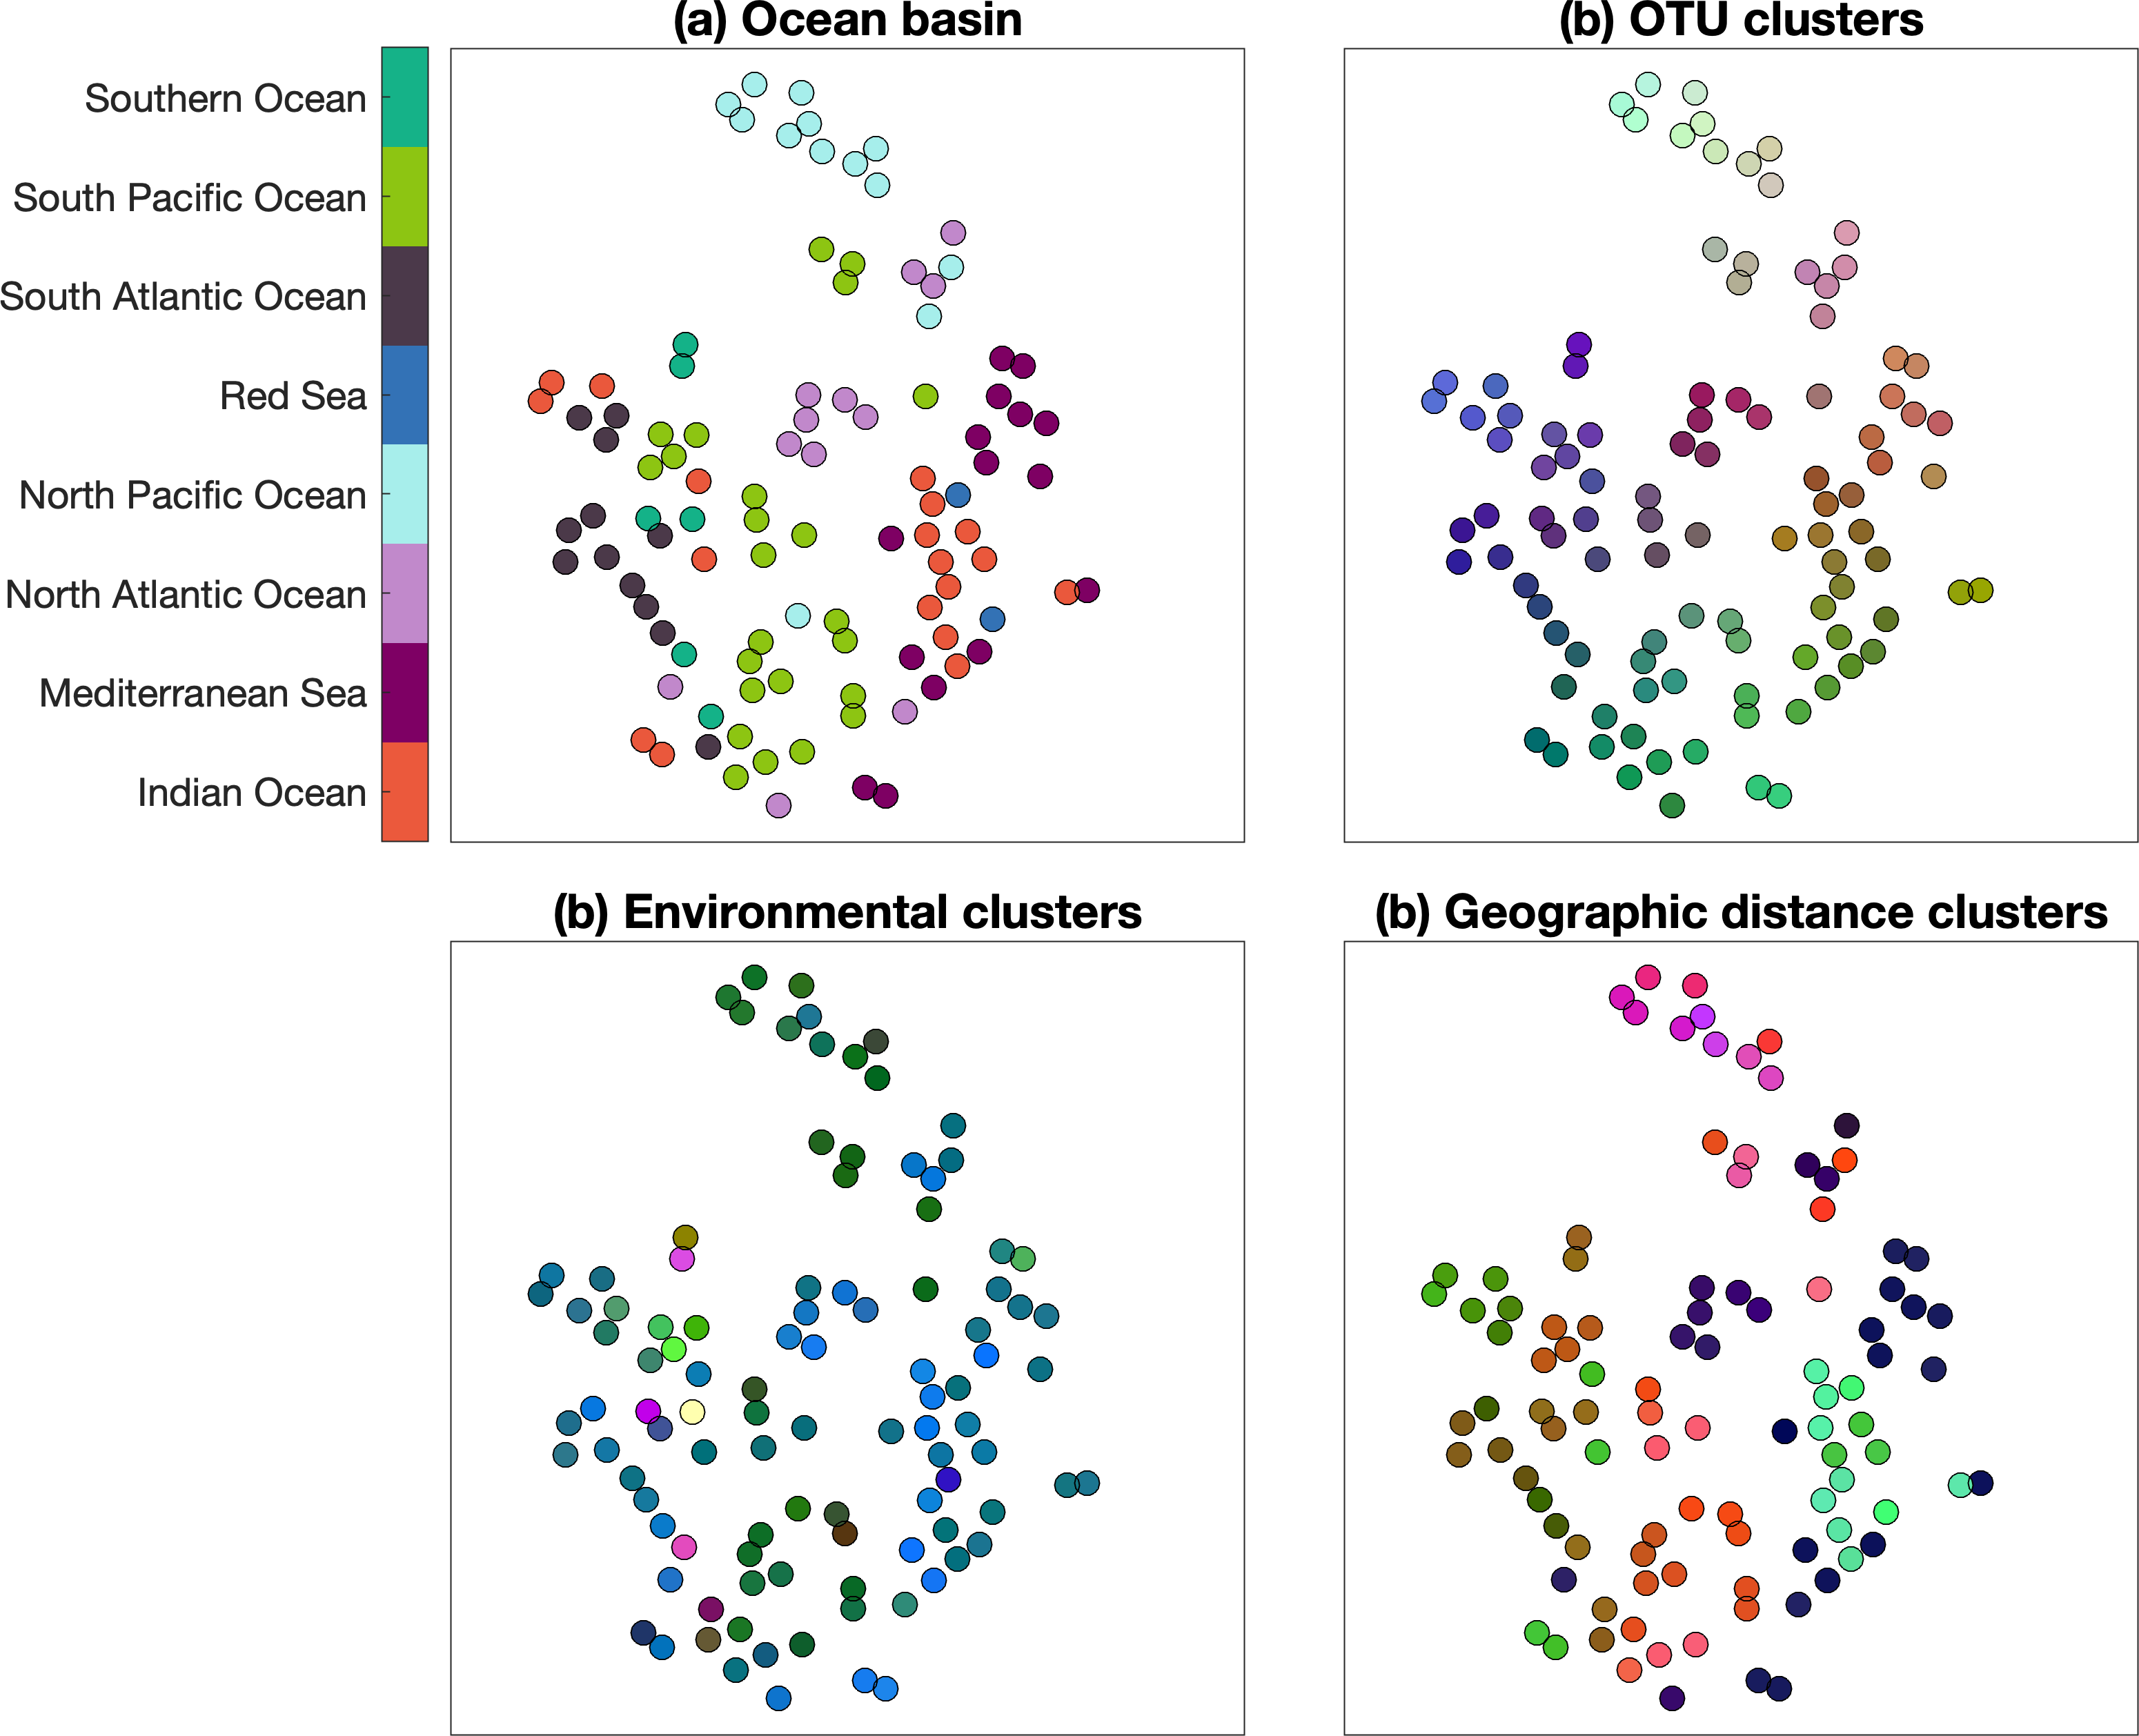
\includegraphics[width=0.75\textwidth]{../Richter_2020_Tara_data/Figures/Martiny_Clusters_OTU_3.png}\
    \caption{}
\label{Tara_HughesMartiny}
\end{figure*}

\begin{figure*}[t!]
    \centering
        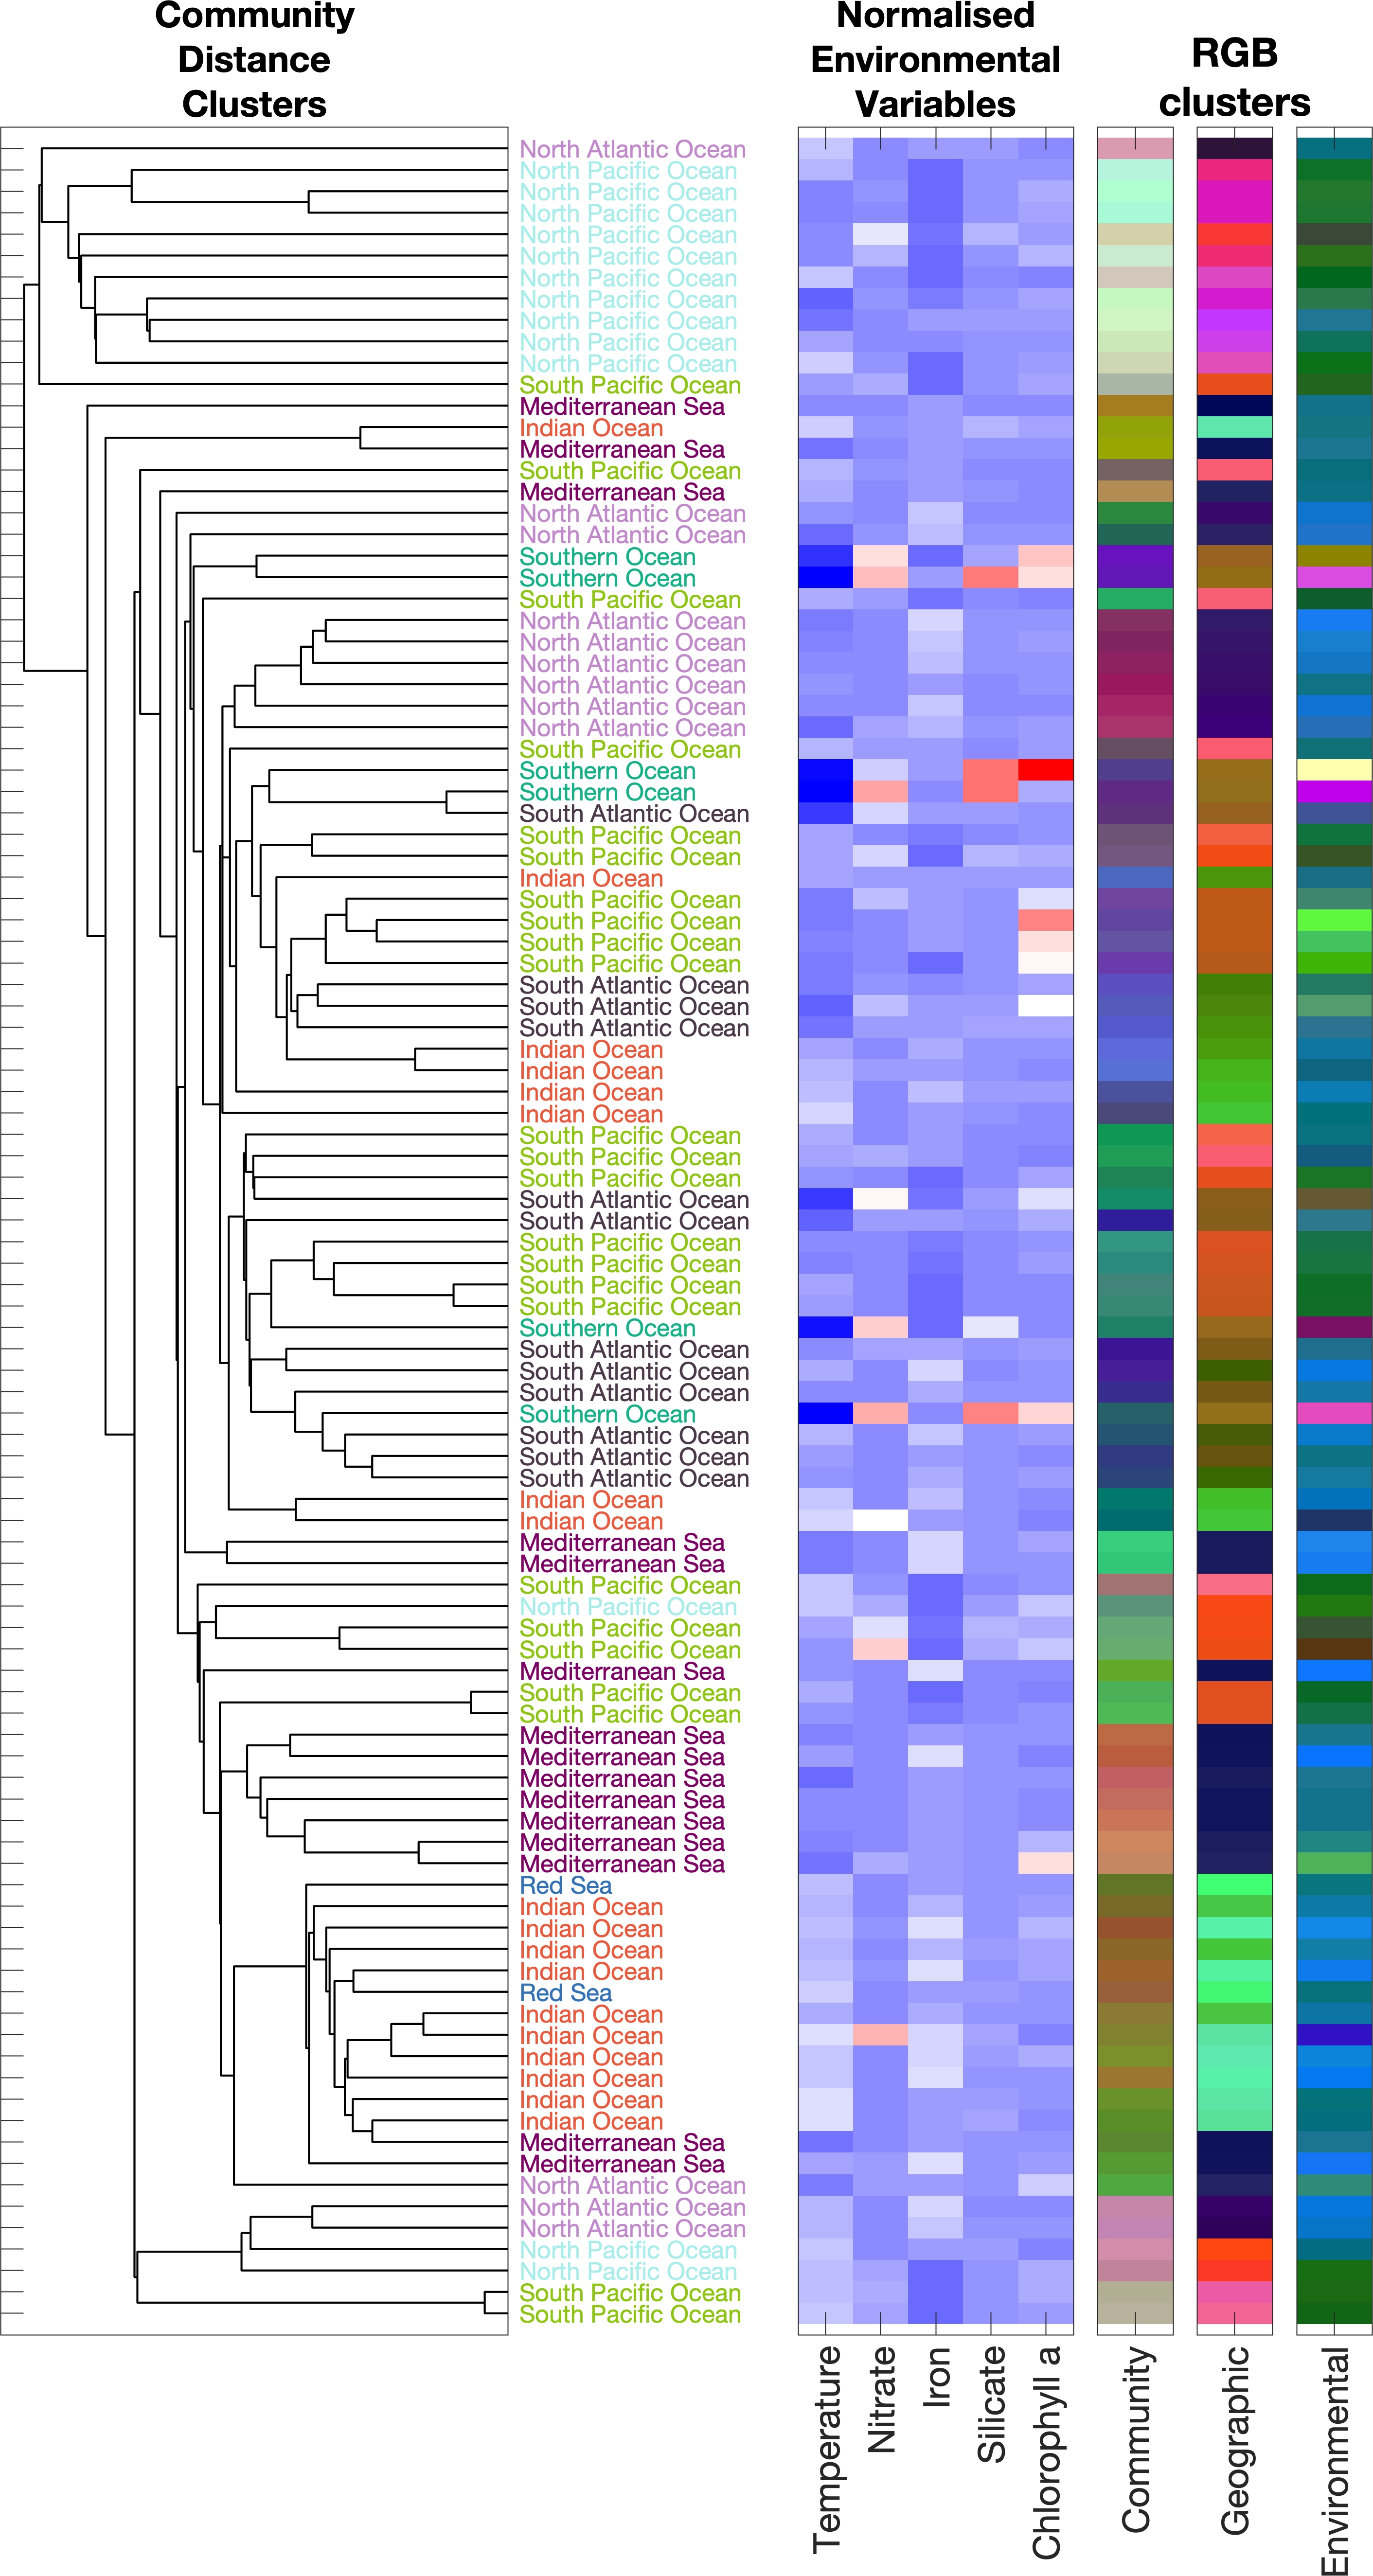
\includegraphics[width=0.8\textwidth]{../Richter_2020_Tara_data/Figures/Dendrogram_OTU_3.png}\
    \caption{}
\label{Tara_Dendrogram}
\end{figure*}


\begin{figure*}[t!]
    \centering
        \includegraphics[width=0.6\textwidth]{../Figures/Figure_3.png}
    \caption{Immigration vs emigration times (years) at the 94 seed locations. The coloured circles show times from the surface-only case. The colour scale indicates absolute latitude, with low latitude regions clearly characterised by fast emigration and slow immigration, with the opposite true at higher latitudes. The black dots show the same time scales in the depth-integrated case.}
\label{Imm_vs_em}
\end{figure*}

\begin{figure*}[htp!]
    \centering
        \includegraphics[width=1\textwidth]{../Figures/abundances-01.png}
\caption{Abundances and cell transport vectors for \textit{Prochlorococcus} (a and c) and diatoms (b and d). The upper panels show transport vectors through the surface layer. The lower panels show depth-integrated transport vectors. We used depth-integrated abundances in all cases.}
\label{Abundances}
\end{figure*}

\begin{figure}[htp!]
\includegraphics[width=1\linewidth]{../Figures/EPMD_Full_cluster_maps.png}
\caption{Community clustering in four simulations. For each experiment (rows), the simmilarity of model communities among sites is indicated by the spatial clustering, as derived using the t-SNE algorithm \citep{VanDerMaaten:2014}. In the first column, sample points are labelled with colours indicating their ocean basin. In the second column, the sample points are coloured according to their environmental similarity, with colder locations coloured blue, and warmer locations coloured red. The third column shows sites coloured by geographic distance, with geographically closer sites having similar colours. The final column shows sites coloured by the same community similarity used to derive their position on the two dimensional axes, but in this case the community similarity was projected into three dimensional space, which was then translated into colour by assigning the three dimensions to red, green and blue colour channels.}
\label{Schematic}
\end{figure}

\end{document}













